\documentclass[conference]{IEEEtran}

\usepackage{cite}
\usepackage{amsmath,amssymb,amsfonts}
\usepackage{algorithmic}
\usepackage{graphicx}
\usepackage{textcomp}
\usepackage{booktabs}
\usepackage{array}
\usepackage{url}
\usepackage{bm}
\usepackage{xcolor}

% Pending result markers
\newcommand{\todo}[1]{{\color{red}\textbf{[TODO: #1]}}}
\newcommand{\pend}{{\color{red}--}}

\begin{document}

\title{Anomaly-Aware Workload Forecasting for Cloud Resource Management}

\author{
\IEEEauthorblockN{
Rohith A. M.,
Shriya Bharadwaj,
Sanskruti Hiwase
}
\IEEEauthorblockA{
Department of Information Technology\\
National Institute of Technology Karnataka, Surathkal, India\\
Course: IT307 Machine Learning
}
}

\maketitle

\begin{abstract}
Cloud providers must decide how much processor and memory capacity future workloads will need. Under-provisioning degrades service, whereas over-provisioning wastes resources. This project first reproduces three forecasting architectures from the literature, namely Long Short-Term Memory (LSTM), probabilistic LSTM (LSTMD), and Hybrid Bayesian Neural Network (HBNN), on Google and Alibaba workload traces. It then asks whether explicit anomaly information helps during sudden workload increases. A multi-signal anomaly detector, combining robust deviation from a rolling median, sudden workload jumps, moving-average residuals, and Isolation Forest predictions, supplies binary flags and continuous severity scores as extra model inputs, and an asymmetric, spike-weighted loss penalizes underprediction more heavily. The experiments use chronological data partitions and eleven workload traces; the LSTM and HBNN results use three random seeds, and the LSTMD results one run per trace.

For the LSTM, severity-score inputs combined with a mild cost-sensitive objective reduce mean paired overall MSE by 7.70\% and spike MSE by 7.82\% relative to raw inputs, while the spike-period underprediction rate rises by 2.38\%. For the probabilistic models the benefit is less consistent. The multi-trace LSTMD is unchanged in accuracy and slightly worse calibrated, and its single-trace S-B configuration gets worse. The multi-trace HBNN improves in accuracy and provisioning cost, although part of that gain comes from unstable raw baselines. None of the models showed a consistent reduction in spike-period underprediction.
\end{abstract}

\begin{IEEEkeywords}
Anomaly detection, cloud computing, LSTM, resource provisioning, service-level metrics, time-series forecasting, workload prediction.
\end{IEEEkeywords}

\section{Introduction}

Cloud computing platforms must allocate computational resources such as CPU and memory according to changing workload demands. Accurate workload forecasting allows cloud providers to allocate resources proactively rather than reacting only after utilization increases.

The consequences of forecasting errors are asymmetric. Underestimating workload demand can result in insufficient computational capacity, increased response times, and violations of service-level agreements. In contrast, overestimating demand results in unnecessary resource allocation and increased operational costs.

Traditional workload forecasting models generally produce point predictions, which provide limited information about the uncertainty associated with future demand. Rossi et al.~\cite{rossi2025} address this limitation through uncertainty-aware forecasting models, including probabilistic LSTM (LSTMD) and Hybrid Bayesian Neural Networks (HBNN). These models estimate predictive uncertainty and allow resource provisioning decisions to be made according to a desired service level.

This project initially reproduces the LSTM, LSTMD, and HBNN architectures proposed in~\cite{rossi2025} using Google and Alibaba workload traces. The reproduced models are evaluated against the results reported in the reference study.

During the reproduction experiments, it was observed that forecasting errors are particularly important during sudden workload increases. These periods can lead to resource under-provisioning and increased service-level violations. This motivates the investigation of anomaly-aware forecasting and cost-sensitive training objectives.

The proposed extension investigates two complementary approaches. First, a multi-signal anomaly detector identifies unusual workload behaviour and generates additional input features. Second, an asymmetric spike-aware loss function assigns higher penalties to underprediction and errors occurring during workload spikes.

The main contributions of this project are:

\begin{enumerate}
\item Reproduction of LSTM, LSTMD, and HBNN forecasting architectures using twelve Google and Alibaba workload traces.

\item Development of a multi-signal anomaly detector combining robust statistical deviation, sudden workload jumps, moving-average residuals, and Isolation Forest predictions.

\item Integration of binary anomaly flags and continuous anomaly severity scores into workload forecasting models.

\item Design of an asymmetric, spike-weighted squared-error objective to reduce underprediction during high-demand periods.

\item Evaluation of forecasting accuracy and resource-provisioning behaviour, using overall and spike-specific metrics, for the LSTM, LSTMD, and HBNN.
\end{enumerate}

The LSTM extension uses point forecasting followed by a validation-calibrated safety margin, whereas the LSTMD and HBNN experiments take their upper bounds from the models' own predictive distributions. The transfer-learning experiments of the original reference work are outside the scope of this project.

The remainder of this paper is organized as follows. Section II reviews related work. Section III describes the reference architectures and their reproduction. Section IV presents the datasets and preprocessing procedure. Section V explains the proposed methodology. Section VI describes the experimental evaluation. Section VII presents the results, discussion, and limitations, and Section VIII concludes the paper.

\section{Related Work}

\subsection{Workload Forecasting}

Workload forecasting has been studied using statistical, machine-learning, and deep-learning approaches. Early studies employed linear time-series models to predict host resource utilization. Dinda and O'Hallaron investigated host-load prediction using statistical models~\cite{dinda2000}, while Calheiros et al. demonstrated the application of ARIMA forecasting for cloud resource provisioning~\cite{calheiros2015}.

Machine-learning approaches have subsequently been used to model more complex workload patterns~\cite{gao2020}. Recurrent neural networks, particularly LSTM architectures, have become widely used because they can capture temporal dependencies in workload sequences~\cite{song2018,bi2021}.

Hybrid convolutional and recurrent architectures have also been investigated for virtual-machine and server workload forecasting~\cite{leka2021,patel2022}. Transformer-based models, including Wasserstein adversarial Transformers, aim to capture longer temporal dependencies~\cite{arbat2022}. Ensemble-based forecasting approaches have also been explored to improve prediction robustness~\cite{kim2020,bao2022}.

\subsection{Uncertainty-Aware Forecasting}

Most conventional forecasting models provide a single predicted value without explicitly representing predictive uncertainty.

Uncertainty-aware forecasting approaches address this limitation through confidence intervals, kernel estimation, quantile regression, and probabilistic neural networks~\cite{minarolli2017,mammen2023}.

Predictive uncertainty is generally divided into two categories:

\begin{itemize}
\item \textbf{Aleatoric uncertainty:} Uncertainty arising from inherent noise and variability in the observed data.

\item \textbf{Epistemic uncertainty:} Uncertainty arising from limited training data and model knowledge.
\end{itemize}

Neural networks can estimate aleatoric uncertainty by predicting the parameters of a probability distribution~\cite{nix1994}. Bayesian neural networks model epistemic uncertainty by placing probability distributions over network weights~\cite{blundell2015}.

Rossi et al.~\cite{rossi2022,rossi2025} investigate uncertainty-aware workload forecasting through probabilistic LSTM and Hybrid Bayesian Neural Network architectures. Their work serves as the primary reference for this project.

\subsection{Anomaly Detection and Cost-Sensitive Forecasting}

Anomaly detection identifies observations that deviate significantly from normal data behaviour. It has been applied to several domains, including network monitoring, fault detection, and time-series analysis~\cite{chandola2009}.

Isolation Forest identifies anomalous observations through random partitioning of the feature space~\cite{liu2008}. Robust statistical methods based on the median absolute deviation provide another approach for detecting unusual observations while reducing sensitivity to extreme values~\cite{leys2013}.

Forecasting errors can also have unequal operational costs. Asymmetric loss functions allow different penalties to be assigned to overprediction and underprediction~\cite{zellner1986}. Quantile regression provides another mechanism for modelling asymmetric prediction objectives~\cite{koenker1978}.

The proposed project combines these ideas by incorporating anomaly information into workload forecasting and applying an asymmetric, spike-weighted training objective.

\section{Reference Models and Reproduction}

\subsection{Forecasting Architectures}

The reference study~\cite{rossi2025} investigates three forecasting architectures:

\begin{enumerate}
\item \textbf{LSTM:} A recurrent neural network that predicts future workload values using historical observations.

\item \textbf{LSTMD:} A probabilistic LSTM that predicts the mean and standard deviation of a Gaussian distribution, allowing it to represent aleatoric uncertainty.

\item \textbf{HBNN:} A Hybrid Bayesian Neural Network that incorporates probabilistic network weights to model epistemic uncertainty in addition to predictive uncertainty.
\end{enumerate}

All three architectures use historical workload observations to predict future CPU and memory utilization.

The input window consists of 288 time steps, corresponding to 24 hours of observations at five-minute intervals. The forecasting horizon is two time steps, corresponding to ten minutes.

The LSTM model uses causal one-dimensional convolutional layers followed by an LSTM layer and fully connected layers. LSTMD uses a similar network structure but produces Gaussian distribution parameters and is trained using negative log-likelihood.

HBNN incorporates a variational Bayesian layer after the initial dense block and uses a probabilistic output layer.

The original study also distinguishes between single-trace and multi-trace training, as well as univariate and bivariate forecasting configurations.

\subsection{Service-Level Metrics}

Uncertainty-aware models can support resource provisioning by estimating an upper prediction bound at a selected confidence or service level.

Let $U_{\gamma}$ denote the upper prediction bound associated with a target service level $\gamma$.

The Service Rate (SR) is defined as the proportion of observations for which actual workload does not exceed the predicted resource capacity:

\begin{equation}
SR =
\frac{1}{N}
\sum_{i=1}^{N}
\mathbb{I}(y_i \leq U_{\gamma,i}).
\end{equation}

The Total Predicted Resources (TPR) represents the total predicted capacity relative to the total actual workload:

\begin{equation}
TPR =
\frac{\sum_{i=1}^{N} U_{\gamma,i}}
{\sum_{i=1}^{N} y_i}
\times 100.
\end{equation}

A smaller TPR at the same SR indicates more efficient resource provisioning.

\subsection{Reproduction Protocol}

The reproduction follows the reference study's experimental structure.

Each workload trace is divided chronologically into training, validation, and test subsets. Approximately 80\% of the observations are allocated to training and validation, while the remaining 20\% are reserved for testing. Of the development portion, 20\% is used for validation.

The input window and forecasting horizon remain consistent with the reference study.

The tuned hyperparameter configurations released with the original implementation are reused where applicable. LSTMD is trained for up to 500 epochs, with the best validation weights restored.

\todo{Confirm random seeds, training epochs for LSTM and HBNN, and the exact hyperparameter configuration used.}

\section{Dataset and Preprocessing}

\subsection{Workload Datasets}

The project uses workload traces from Google Cluster datasets and Alibaba Cluster datasets.

The traces represent CPU and memory utilization collected from cloud computing environments. The datasets are aggregated into five-minute intervals to obtain consistent time-series observations.

Table~\ref{tab:traces} summarizes the workload traces used in the reproduction and anomaly-aware extension.

\begin{table}[!t]
\caption{Workload Traces Used in the Project}
\label{tab:traces}
\centering
\footnotesize
\begin{tabular}{p{0.22\columnwidth}p{0.35\columnwidth}p{0.22\columnwidth}}
\toprule
\textbf{Source} & \textbf{Traces} & \textbf{Points}\\
\midrule
Google 2011 & gc11 & 8,352\\
Google 2019 & gc19\_a--h & 8,352 each\\
Alibaba 2018 & ali18 & About 2,000\\
Alibaba 2020 & ali20\_c, ali20\_g & 13,904 each\\
\bottomrule
\end{tabular}
\end{table}

The reproduction experiments use all twelve traces. The anomaly-aware extension uses eleven traces, excluding the shorter Alibaba 2018 trace.

This exclusion provides a more consistent validation partition for estimating anomaly thresholds and calibrating the resource safety margin.

\subsection{Data Preprocessing}

The preprocessing procedure consists of the following steps:

\begin{enumerate}
\item Aggregate raw workload observations into five-minute intervals.

\item Calculate average CPU and memory utilization for each interval.

\item Remove missing and infinite observations.

\item Forward-fill gaps in the workload series and use training-set median values for any remaining missing observations.

\item Apply min-max scaling to normalize CPU and memory utilization to the range $[0,1]$.
\end{enumerate}

The resulting dataset contains two workload signals: CPU utilization and memory utilization.

\subsection{Chronological Data Partitioning}

For the anomaly-aware extension, each trace is divided chronologically into three subsets:

\begin{itemize}
\item Training: 70\%
\item Validation: 10\%
\item Testing: 20\%
\end{itemize}

A forecasting window is assigned to a partition according to the timestamp of its target observation. This ensures that validation and test targets occur after the training targets.

Anomaly detection thresholds, Isolation Forest parameters, and spike thresholds are estimated using training data only.

The validation set is used for model selection and resource safety-margin calibration, while the test set is reserved for final evaluation.

The LSTMD and HBNN experiments use a different chronological split, 64\% training, 16\% validation and 20\% test, and obtain their upper bounds from the predictive distribution instead of a validation-calibrated margin (Sections~\ref{sec:lstmd_results} and~\ref{sec:hbnn_results}).

\section{Proposed Methodology}

The proposed framework integrates anomaly-aware feature extraction and cost-sensitive training into workload forecasting.

The framework consists of four major stages:

\begin{enumerate}
\item Workload preprocessing and normalization.
\item Multi-signal anomaly detection.
\item LSTM, LSTMD, and HBNN workload forecasting.
\item Cost-sensitive training and service-level evaluation.
\end{enumerate}

\subsection{Multi-Signal Anomaly Detection}

Workload traces may contain sudden increases, irregular fluctuations, and unusual utilization patterns. Detecting these events can provide additional information to forecasting models.

The proposed anomaly detector combines four complementary detection signals.

\subsubsection{Robust Z-Score}

The robust Z-score measures the deviation of an observation from its rolling median.

It is calculated using the median absolute deviation (MAD):

\begin{equation}
R_t =
\frac{x_t-\operatorname{Median}(x)}
{1.4826 \times MAD(x)+\epsilon}.
\end{equation}

Here, $x_t$ represents the current workload observation and $\epsilon$ prevents division by zero.

\subsubsection{Jump Z-Score}

The jump detector identifies sudden workload changes using first-order differences:

\begin{equation}
d_t=x_t-x_{t-1}.
\end{equation}

The jump Z-score measures the magnitude of this change relative to a robust scale estimated from historical differences.

\subsubsection{EMA Residual}

The exponential moving average captures the recent workload trend.

The residual is calculated as:

\begin{equation}
r_t=x_t-EMA_t.
\end{equation}

A large residual indicates that the current workload differs significantly from its recent trend.

\subsubsection{Isolation Forest}

Isolation Forest identifies observations that exhibit unusual patterns in the derived feature space.

The detector is fitted using training observations only and subsequently applied to validation and test observations.

\subsubsection{Anomaly Voting and Severity}

Let the four detector outputs be represented by:

\begin{equation}
v_{R,t},v_{J,t},v_{E,t},v_{I,t}.
\end{equation}

The binary anomaly flag is generated using a voting mechanism:

\begin{equation}
f_t =
\mathbb{I}
\left[
\sum_{k\in\{R,J,E,I\}}v_{k,t}
\geq 2
\land R_t>0
\right].
\end{equation}

The additional positive robust-score condition ensures that the final flag emphasizes unusual upward workload behaviour.

A continuous severity score $q_t\in[0,1]$ is also generated by averaging normalized detector strengths.

The binary flag represents a thresholded anomaly decision, whereas the continuous score preserves information about the degree of unusual workload behaviour.

Both outputs are calculated independently for CPU and memory.

\begin{figure}[!t]
\centering
\includegraphics[width=\columnwidth]{anomaly_detection_pipeline.png}
\caption{Multi-signal anomaly detection and feature generation.}
\label{fig:detector}
\end{figure}

\subsection{Forecasting Architectures}

The proposed anomaly-aware features are integrated into three forecasting architectures: LSTM, LSTMD, and HBNN.

Each model receives a historical workload window containing 288 time steps.

The baseline input consists of CPU and memory utilization:

\begin{equation}
X_t=[CPU_t,Memory_t].
\end{equation}

For anomaly-aware configurations, additional channels are appended to the original workload features.

These include:

\begin{itemize}
\item Binary anomaly flags for CPU and memory.
\item Continuous anomaly severity scores for CPU and memory.
\item Both binary flags and continuous severity scores.
\end{itemize}

The anomaly features provide additional historical information that may help the forecasting models identify unusual workload behaviour.

The LSTM architecture serves as the recurrent baseline, while LSTMD and HBNN provide probabilistic forecasting architectures for investigating whether the proposed enhancements generalize across different model structures.

The LSTM ablation in Section~VII uses an enlarged version of the reference network: a causal residual convolution block with layer normalization, a bidirectional LSTM over the observed 288-step window (it never sees target or future samples), temporal attention pooling, dropout, and learning-rate reduction on plateau. Input features and targets are standardized with training statistics only.

\begin{figure}[!t]
\centering
\includegraphics[width=\columnwidth]{lstm_architecture.png}
\caption{LSTM forecasting architecture with anomaly-aware inputs.}
\label{fig:lstm}
\end{figure}

\begin{figure}[!t]
\centering
\includegraphics[width=\columnwidth]{hbnn_architecture.png}
\caption{Hybrid Bayesian Neural Network (HBNN) forecasting architecture.}
\label{fig:hbnn}
\end{figure}

\subsection{Asymmetric and Spike-Aware Loss Function}

The second proposed enhancement modifies the training objective to account for the unequal consequences of overprediction and underprediction.

Let $y_i^{(r)}$ represent the actual workload and $\hat{y}_i^{(r)}$ represent the predicted workload for resource $r$.

The prediction error is:

\begin{equation}
e_i^{(r)}=y_i^{(r)}-\hat{y}_i^{(r)}.
\end{equation}

A positive error indicates underprediction, which may result in insufficient resource allocation.

A binary spike indicator $s_i^{(r)}$ identifies workload increases relative to the previous observation. The spike threshold is estimated using the 95th percentile of positive workload changes in the training data.

The proposed asymmetric, spike-weighted objective is:

\begin{equation}
\mathcal{L} =
\frac{1}{2N}
\sum_{i=1}^{N}\sum_r
w_i^{(r)}(e_i^{(r)})^2
\end{equation}

where

\begin{equation}
w_i^{(r)} =
\left[
1+(\alpha-1)\mathbb{I}(e_i^{(r)}>0)
\right]
\left[
1+\lambda s_i^{(r)}
\right].
\end{equation}

Here, $\alpha\geq1$ controls the additional penalty for underprediction, while $\lambda\geq0$ controls the additional weight assigned to spike observations.

When $\alpha=1$ and $\lambda=0$, the objective reduces to ordinary mean squared error.

Increasing $\alpha$ makes underprediction more expensive, while increasing $\lambda$ emphasizes errors occurring during workload spikes.

The spike indicator is used only during training and is not provided as a future input to the forecasting model.

The experiments investigate standard MSE, Huber loss, and asymmetric spike-aware configurations where implemented.

\begin{figure*}[!t]
\centering
\includegraphics[width=0.92\textwidth]{cost_sensitive_loss_pipeline.png}
\caption{Asymmetric and spike-aware training objective.}
\label{fig:loss}
\end{figure*}

\subsection{Experimental Design and Ablation Study}

The experimental design evaluates the independent and combined contributions of anomaly-aware features and cost-sensitive training.

The input configurations include:

\begin{enumerate}
\item Raw workload features.
\item Raw features augmented with anomaly flags.
\item Raw features augmented with anomaly severity scores.
\item Raw features augmented with both flags and scores.
\end{enumerate}

The training objectives include:

\begin{enumerate}
\item Standard mean squared error.
\item Huber loss.
\item Asymmetric loss with different underprediction penalties.
\item Asymmetric spike-weighted loss.
\end{enumerate}

These comparisons investigate whether anomaly-aware inputs improve prediction accuracy, whether asymmetric training reduces underprediction, and whether combining both approaches provides additional benefits.

The anomaly-aware inputs are also tested on the probabilistic LSTMD and HBNN, to see whether the effect seen in the LSTM carries over. Those runs use the Gaussian negative log-likelihood, so the asymmetric loss is not applied to them.

For the LSTM experiments, an initial screening stage uses validation performance to identify promising configurations. Selected configurations are subsequently evaluated across the complete extension dataset.

\section{Experimental Evaluation}

\subsection{Training Protocol}

The forecasting models are trained using chronological data partitions.

Each input sequence contains 288 historical time steps, and the prediction horizon is two time steps.

Training and model selection are performed using training and validation observations, respectively. The test observations are reserved for final evaluation.

Feature scaling parameters, anomaly thresholds, and spike thresholds are estimated using training data only.

Multiple random seeds are used to assess the stability of the selected configurations.

For resource provisioning, a safety margin is estimated from validation residuals and applied to the point forecasts.

\subsection{Point-Forecast Metrics}

The following metrics are used to evaluate forecasting accuracy.

\subsubsection{Mean Squared Error}

\begin{equation}
MSE=\frac{1}{N}\sum_{i=1}^{N}(y_i-\hat{y}_i)^2.
\end{equation}

MSE penalizes larger prediction errors more heavily.

\subsubsection{Mean Absolute Error}

\begin{equation}
MAE=\frac{1}{N}\sum_{i=1}^{N}|y_i-\hat{y}_i|.
\end{equation}

MAE measures the average absolute difference between actual and predicted workload.

\subsubsection{Spike MSE}

Spike MSE measures prediction error specifically during workload spike observations:

\begin{equation}
MSE_{spike}=
\frac{\sum_i s_i(y_i-\hat{y}_i)^2}
{\sum_i s_i}.
\end{equation}

\subsubsection{Underprediction Rate}

The underprediction rate measures the proportion of observations for which actual workload exceeds predicted workload:

\begin{equation}
U_R=
\frac{1}{N}
\sum_{i=1}^{N}
\mathbb{I}(y_i>\hat{y}_i).
\end{equation}

\subsubsection{Mean Spike Shortfall}

Mean spike shortfall measures the average magnitude of underprediction during spike periods:

\begin{equation}
SS=
\frac{\sum_i s_i\max(0,y_i-\hat{y}_i)}
{\sum_i s_i}.
\end{equation}

\subsection{Service-Level Evaluation}

The forecasting models are further evaluated according to resource-provisioning behaviour.

For the anomaly-aware point forecasters, a safety margin is estimated using validation residuals:

\begin{equation}
U_{\gamma,i}=\hat{y}_i+Q_{\gamma}(r_{val}),
\end{equation}

where $Q_{\gamma}(r_{val})$ denotes the selected quantile of validation residuals.

The upper capacity bound is then used to calculate service-level success rate and total predicted resources.

The evaluation considers the following measures:

\begin{itemize}
\item Overall Service Rate (SR).
\item Spike-specific Service Rate.
\item Total Predicted Resources (TPR).
\item Resource-provisioning efficiency at selected service levels.
\end{itemize}

The experiments consider target service levels of 95\% and 99\%, among others.

For the LSTM ablation in Table~\ref{tab:point} only point-error metrics were exported, so SR and TPR are reported for the LSTMD and HBNN, whose upper bounds come from their predictive distributions, and not for the LSTM.

\section{Results and Analysis}

\subsection{Reproduction of Reference Models}

Table~\ref{tab:repro} compares the published accuracy values of Rossi et al.~\cite{rossi2025} with the corresponding reproduced results.

The evaluation considers twelve configurations involving LSTM, LSTMD, and HBNN architectures, including univariate, bivariate, single-trace, and multi-trace settings.

\begin{table*}[!t]
\caption{Reproduction of the Forecasting Accuracy Results. The reproduced LSTMD values are means over eleven traces; the LSTM and HBNN rows are still to be filled in.}
\label{tab:repro}
\centering
\footnotesize
\begin{tabular}{lcccc|cccc}
\toprule
& \multicolumn{4}{c|}{\textbf{Reported Results}}
& \multicolumn{4}{c}{\textbf{Reproduced Results}}\\
\textbf{Model}
& CPU MSE & CPU MAE & Mem. MSE & Mem. MAE
& CPU MSE & CPU MAE & Mem. MSE & Mem. MAE\\
\midrule
S-U-LSTM  & 0.0041 & 0.0457 & 0.0042 & 0.0425 & \pend & \pend & \pend & \pend\\
S-U-LSTMD & 0.0040 & 0.0455 & 0.0041 & 0.0420 & 0.0032 & 0.0396 & 0.0046 & 0.0457\\
S-U-HBNN  & 0.0047 & 0.0502 & 0.0044 & 0.0455 & \pend & \pend & \pend & \pend\\
S-B-LSTM  & 0.0047 & 0.0500 & 0.0054 & 0.0487 & \pend & \pend & \pend & \pend\\
S-B-LSTMD & 0.0061 & 0.0556 & 0.0088 & 0.0631 & 0.0032 & 0.0400 & 0.0032 & 0.0367\\
S-B-HBNN  & 0.0299 & 0.1285 & 0.0386 & 0.1533 & \pend & \pend & \pend & \pend\\
M-U-LSTM  & 0.0044 & 0.0474 & 0.0048 & 0.0447 & \pend & \pend & \pend & \pend\\
M-U-LSTMD & 0.0041 & 0.0464 & 0.0044 & 0.0439 & 0.0031 & 0.0393 & 0.0030 & 0.0353\\
M-U-HBNN  & 0.0047 & 0.0485 & 0.0052 & 0.0498 & \pend & \pend & \pend & \pend\\
M-B-LSTM  & 0.0044 & 0.0479 & 0.0044 & 0.0438 & \pend & \pend & \pend & \pend\\
M-B-LSTMD & 0.0046 & 0.0446 & 0.0046 & 0.0446 & 0.0031 & 0.0393 & 0.0030 & 0.0359\\
M-B-HBNN  & 0.0042 & 0.0471 & 0.0043 & 0.0436 & \pend & \pend & \pend & \pend\\
\bottomrule
\end{tabular}
\end{table*}

For LSTMD, the reproduced errors are at or below the reported values in 14 of the 16 entries. The exceptions are the S-U memory MSE and MAE (0.0046 and 0.0457 against 0.0041 and 0.0420). That mean is inflated by a single series: the raw S-U model for gc19\_e memory stopped improving after three epochs and reaches a test MSE of 0.0198, so we read it as a failed fit and not as a systematic gap. The comparison is not strictly like-for-like, because the reproduced LSTMD values cover eleven of the twelve traces of the reference study.

\todo{Fill in the reproduced LSTM and HBNN rows of Table~\ref{tab:repro} and discuss how they agree with the reported values.}

\subsection{Point Accuracy of Anomaly-Aware Variants}

The completed LSTM ablation evaluates four configurations on eleven workload traces, using three random seeds and both CPU and memory targets. This corresponds to 132 final model fits (11 traces $\times$ 4 configurations $\times$ 3 seeds), producing 264 trace/configuration/seed/resource test rows across CPU and memory. The configurations compare raw features, severity-score features, and the addition of a mild cost-sensitive objective. The anomaly-aware experiments compare the forecasting performance of different input and loss configurations.

Table~\ref{tab:point} reports the evaluation metrics as ratios relative to the baseline model. Values below one indicate improvements over the baseline.

\begin{table*}[!t]
\caption{LSTM Anomaly-Aware Ablation: Mean Paired Test-Metric Ratios Relative to the Raw-Feature MSE Baseline}
\label{tab:point}
\centering
\footnotesize
\begin{tabular}{lcccccc}
\toprule
\textbf{Configuration} & \textbf{MSE} & \textbf{MAE} &
\textbf{Spike MSE} & \textbf{Spike MAE} &
\textbf{Underpred. Rate} & \textbf{Spike Underpred. Rate}\\
\midrule
raw\_mse      & 1.0000 & 1.0000 & 1.0000 & 1.0000 & 1.0000 & 1.0000\\
score\_mse    & 0.9449 & 0.9553 & 0.9634 & 0.9698 & 0.9645 & 1.0237\\
score\_mild1  & \textbf{0.9230} & \textbf{0.9366} & \textbf{0.9218} & \textbf{0.9444} & \textbf{0.9267} & 1.0238\\
all\_mse      & 0.9346 & 0.9492 & 0.9971 & 0.9919 & 1.0061 & 1.0657\\
\bottomrule
\end{tabular}
\end{table*}

The LSTM ablation evaluates four configurations: raw workload features with MSE (\texttt{raw\_mse}), anomaly severity scores with MSE (\texttt{score\_mse}), anomaly severity scores with a mild cost-sensitive objective (\texttt{score\_mild1}), and binary anomaly flags together with severity scores using MSE (\texttt{all\_mse}). The ratios are computed by pairing each configuration with the raw-feature baseline for the same trace, random seed, data split, and resource. Values below one indicate lower error or a lower underprediction rate; values above one indicate an increase.

The final LSTM test evaluation covers eleven traces, three random seeds, and CPU and memory targets. The selected \texttt{score\_mild1} configuration achieves the strongest aggregate trade-off: overall MSE decreases by 7.70\%, overall MAE by 6.34\%, spike MSE by 7.82\%, and spike MAE by 5.56\%. Its overall underprediction rate also decreases by 7.33\%. However, its spike-period underprediction rate is 2.38\% higher than the baseline. Therefore, the results support improved average forecasting accuracy, but do not establish a reduction in spike-period underprediction frequency. The gain is also not uniform across traces: \texttt{score\_mild1} lowers overall MSE on 8 of the 11 traces, and a bootstrap over traces gives a 95\% interval of 0.78--1.05 for its mean MSE ratio, which includes one.

The \texttt{score\_mse} configuration also improves the four error metrics and overall underprediction rate, although less than \texttt{score\_mild1}. In contrast, \texttt{all\_mse} provides only a small improvement in overall errors and almost no improvement in spike-specific errors; its overall and spike-period underprediction rates increase. This suggests that adding both binary flags and severity scores is not automatically better than using severity scores alone.

The ratios summarize paired comparisons across trace, seed, and resource. They should not be interpreted as absolute MSE or MAE values, and the aggregate does not imply that every individual trace improves. Service-level metrics were not exported for these LSTM runs, so SR and TPR are reported for the LSTMD and HBNN below.

\begin{figure}[!t]
\centering
\includegraphics[width=\columnwidth]{01_error_metric_ratios.png}
\caption{Mean paired ratios of overall and spike-specific test errors for the LSTM anomaly-aware configurations, normalized against the raw-feature MSE baseline. Values below one indicate improvement.}
\label{fig:lstm_error_ratios}
\end{figure}

\begin{figure}[!t]
\centering
\includegraphics[width=\columnwidth]{02_underprediction_ratios.png}
\caption{Mean paired ratios of overall and spike-period underprediction rates relative to the raw-feature MSE baseline. Values above one indicate an increase in underprediction frequency.}
\label{fig:lstm_underprediction}
\end{figure}

\subsection{Anomaly-Aware LSTMD}
\label{sec:lstmd_results}

The same question was asked of the probabilistic LSTM. We trained LSTMD with raw inputs and with anomaly-aware inputs on the same eleven traces, using the same chronological split as the HBNN (64\% training, 16\% validation, 20\% test) and the Gaussian negative log-likelihood, so the asymmetric loss is not used here. Each model was trained for up to 500 epochs with the best validation weights restored, and both variants reuse the same tuned hyperparameter sets released with the reference implementation, chosen per configuration and trace. The upper bound at target level $\gamma$ is the predicted mean plus $z_\gamma$ times the predicted standard deviation, so it reflects aleatoric uncertainty only. One run was made per configuration, trace, and variant (72 fits: 36 raw and 36 anomaly-aware; the univariate models are trained separately for CPU and memory), so there is no seed-to-seed spread and the numbers below are descriptive. \todo{Confirm the LSTMD anomaly input channels, the loss, and the spike label (about 11\% of test points are labelled as spikes).}

\textit{Point accuracy.}
Table~\ref{tab:lstmd_acc} and Fig.~\ref{fig:lstmd_summary}(a) give the point-forecast results. In the multi-trace configurations the anomaly inputs change little. The paired MSE ratio, anomaly-aware over raw, is 1.002 for M-U and 0.993 for M-B, the MAE ratios are 1.003 and 0.999, and the anomaly-aware model is better on 7 and 5 of the 11 traces respectively. The single-trace configurations are worse or mixed. S-B gets worse (MSE ratio 1.104, a bootstrap over traces gives a 95\% interval of 1.02--1.21, and only 4 of 11 traces improve), and S-U is worse for CPU (1.075) and about unchanged for memory (0.986). The large drop in S-U memory MSE in Table~\ref{tab:lstmd_acc} (0.0046 to 0.0030) is not an effect of the inputs. It comes from one trace, gc19\_e, where the raw memory model failed (see the reproduction above) and the anomaly-aware one did not. The anomaly inputs therefore do not give LSTMD a consistent accuracy gain.

\textit{Spikes.}
Fig.~\ref{fig:lstmd_summary}(a) and the right half of Table~\ref{tab:lstmd_acc} look at the spike points. The effects are small and mixed. Spike MSE is about 4\% lower for M-U on both resources and 19\% lower for M-B memory, but 6\% higher for M-B CPU, and the single-trace models move by 5\% or less. In the multi-trace models the mean forecast lies below the actual value at about 99\% of spike points with and without the anomaly inputs. As with the HBNN, the network gets closer to the spike but almost always still lands under it. The overall underprediction rate of M-B does fall, from 53.7\% to 48.4\% of points, but that shift does not reach the spikes.

\textit{Service level.}
Table~\ref{tab:lstmd_service} and Fig.~\ref{fig:lstmd_summary}(b,c) show the upper bound. For the multi-trace models and S-B, coverage and cost are nearly identical with and without the anomaly inputs. At the 95\% target the multi-trace models reach an SR of about 95\% at a TPR of 113--115\%, and at the 99\% target about 98.2\% at 120--121\%. The inputs make calibration slightly worse, not better: the mean gap grows from 0.69 to 1.48 percentage points for M-B and from 0.61 to 0.99 for M-U. In every configuration the realised SR is above the target at the low levels and falls short at the highest ones (98.2\% at the 99\% target). For S-U the raw model needs a TPR of 121.7\% at the 95\% target against 113.4\% for the anomaly-aware one. This is again the failed gc19\_e memory fit, whose very large predicted variance inflates the bound (TPR of 290\%). Without that series the two are 113.7\% and 113.4\%, and the raw SR is 0.9 points higher.

Both probabilistic models used the same split, so one comparison is worth making. The raw multi-trace LSTMD already reaches an SR of 95.1\% at a TPR of 114.8\% for M-B, close to the anomaly-aware HBNN (95.8\% at 116.4\%) and much more efficient than the raw HBNN (93.7\% at 129.4\%). The HBNN used one shared, untuned hyperparameter set while LSTMD used the tuned sets from the reference, so this is not a clean architecture comparison. It is consistent with reading part of the HBNN gain from the anomaly inputs as the repair of a weak raw baseline.

\begin{table*}[!t]
\caption{LSTMD with and without anomaly-aware inputs, mean over 11 traces (one run per trace). Spike under-prediction is the share of spike points where the mean forecast lies below the actual demand. Lower is better in every column; the better value of each pair is in bold.}
\label{tab:lstmd_acc}
\centering
\footnotesize
\setlength{\tabcolsep}{4.5pt}
\begin{tabular}{llcccccccc}
\toprule
 & & \multicolumn{2}{c}{MSE} & \multicolumn{2}{c}{MAE} & \multicolumn{2}{c}{Spike MSE} & \multicolumn{2}{c}{Spike under-pred. (\%)}\\
\cmidrule(lr){3-4}\cmidrule(lr){5-6}\cmidrule(lr){7-8}\cmidrule(lr){9-10}
Config. & Res. & Raw & Anomaly & Raw & Anomaly & Raw & Anomaly & Raw & Anomaly\\
\midrule
S-U & CPU & \textbf{0.0032} & 0.0035 & \textbf{0.040} & 0.042 & \textbf{0.0103} & 0.0106 & 99.5 & \textbf{98.8}\\
 & Mem. & 0.0046 & \textbf{0.0030} & 0.046 & \textbf{0.036} & 0.0099 & \textbf{0.0090} & \textbf{90.4} & 99.1\\
\addlinespace[2pt]
S-B & CPU & \textbf{0.0032} & 0.0036 & \textbf{0.040} & 0.043 & 0.0089 & \textbf{0.0086} & 97.1 & \textbf{94.7}\\
 & Mem. & \textbf{0.0032} & 0.0036 & \textbf{0.037} & 0.040 & \textbf{0.0088} & 0.0092 & 97.5 & 97.5\\
\addlinespace[2pt]
M-U & CPU & 0.0031 & 0.0031 & 0.039 & 0.039 & 0.0119 & \textbf{0.0112} & 99.6 & \textbf{99.5}\\
 & Mem. & 0.0030 & \textbf{0.0029} & 0.035 & 0.035 & 0.0096 & \textbf{0.0094} & \textbf{99.0} & 99.2\\
\addlinespace[2pt]
M-B & CPU & 0.0031 & \textbf{0.0030} & 0.039 & 0.039 & \textbf{0.0099} & 0.0104 & \textbf{98.2} & 98.8\\
 & Mem. & 0.0030 & 0.0030 & 0.036 & 0.036 & 0.0094 & \textbf{0.0080} & \textbf{98.7} & 98.9\\
\bottomrule
\end{tabular}
\end{table*}

\begin{figure*}[!t]
\centering
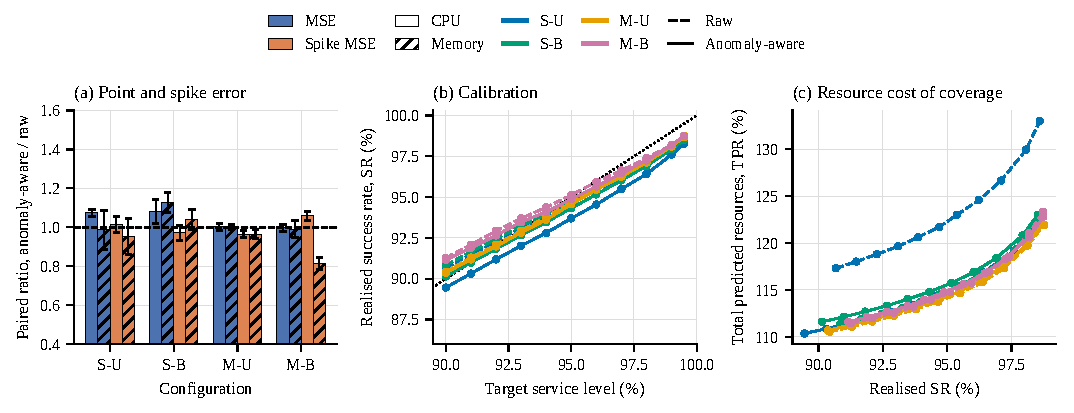
\includegraphics[width=\textwidth]{lstmd_fig_summary.pdf}
\caption{LSTMD with raw and anomaly-aware inputs. (a) Paired ratio of overall MSE and spike MSE, anomaly-aware over raw, for CPU and memory; values below one favour the anomaly-aware inputs, and error bars show the standard error over 11 traces. (b) Realised success rate against the target service level, averaged over CPU and memory; the dotted diagonal is perfect calibration. (c) Total predicted resources against realised SR. Dashed lines are raw inputs and solid lines anomaly-aware inputs.}
\label{fig:lstmd_summary}
\end{figure*}

\begin{table}[!t]\caption{Service-level behaviour of the LSTMD upper bound (mean over CPU, memory and 11 traces, one run per trace). SR is the realised success rate, TPR the total predicted resources as a percentage of actual demand, and Cal.\ the mean absolute gap between realised and target SR over the eleven target levels from 90\% to 99.5\%.}
\label{tab:lstmd_service}
\centering
\footnotesize
\setlength{\tabcolsep}{3.6pt}
\begin{tabular}{llccccc}
\toprule
 & & \multicolumn{2}{c}{95\% target} & \multicolumn{2}{c}{99\% target} & Cal.\\
\cmidrule(lr){3-4}\cmidrule(lr){5-6}
Config. & Input & SR & TPR & SR & TPR & (pp)\\
\midrule
S-U & Raw & 94.7 & 121.7 & 98.1 & 130.0 & 1.06\\
 & Anomaly & 93.7 & 113.4 & 97.6 & 119.2 & 1.21\\
\addlinespace[2pt]
S-B & Raw & 94.7 & 114.5 & 98.0 & 120.5 & 0.62\\
 & Anomaly & 94.3 & 114.8 & 97.9 & 120.8 & 0.70\\
\addlinespace[2pt]
M-U & Raw & 94.7 & 113.7 & 98.1 & 119.7 & 0.61\\
 & Anomaly & 94.6 & 113.9 & 98.1 & 119.8 & 0.99\\
\addlinespace[2pt]
M-B & Raw & 95.1 & 114.8 & 98.2 & 121.1 & 0.69\\
 & Anomaly & 94.9 & 114.7 & 98.2 & 120.6 & 1.48\\
\bottomrule
\end{tabular}
\end{table}

\subsection{Anomaly-Aware HBNN}
\label{sec:hbnn_results}

The ablation above uses a point forecaster. To see whether the anomaly inputs also matter for a probabilistic model, we trained the HBNN with and without them on the same eleven traces. The setup differs from the LSTM study in a few ways that matter when reading the numbers. In the anomaly-aware variant each resource is given its workload channel together with its binary flag and its severity score, so a univariate model sees three channels and a bivariate model six. The loss is the Gaussian negative log-likelihood, so there is no asymmetric or spike weighting here. Windows were split chronologically by target time into 64\% training, 16\% validation and 20\% test. One hyperparameter set, taken from the reference M-B configuration (a convolution with 16 filters of width 3, an LSTM with 32 units, two dense layers of 32 units and a Bayesian dense layer with 8 units), was used for all four configurations, and no hyperparameter search was run. Four configurations, two input variants, eleven traces and three seeds give 216 fits. Predictive uncertainty comes from 100 stochastic forward passes: the aleatoric part is the mean predicted variance, the epistemic part is the variance of the predicted means across passes, and the upper bound at target level $\gamma$ is the mean plus $z_\gamma$ times the square root of the total variance. Because of these differences the raw HBNN numbers below are not an exact reproduction of~\cite{rossi2025}, and they should not be compared directly with the LSTM results.

\textit{Point accuracy.}
Table~\ref{tab:hbnn_acc} and Fig.~\ref{fig:hbnn_acc} give the point-forecast results. In the multi-trace configurations the anomaly inputs lower the CPU MSE from 0.0198 to 0.0031 for both M-U and M-B, and the memory MSE of M-B from 0.0179 to 0.0031. M-U memory is the exception: the two variants are indistinguishable at 0.0029. For the single-trace configurations the picture is mixed. S-B improves by about 20--23\% in MSE, while S-U is unchanged for CPU and about 11\% lower for memory. The paired ratios in Fig.~\ref{fig:hbnn_ratio} tell the same story, but the error bars of the single-trace models are wide (for example an MSE ratio of 1.43 for S-U CPU with a standard error of about 0.3), so we do not read those as a consistent gain or loss.

We are careful with the large gains of the multi-trace models. The raw M-U CPU and M-B models vary a lot between runs (an MSE standard deviation of 0.0276 around a mean of 0.0198), while the raw M-U memory model, trained in the same way, reaches 0.0029. This suggests that part of the gap comes from unstable training of the raw models and not from the anomaly inputs alone. We did not check run by run which fits drive it, so the safest statement is that the anomaly-aware multi-trace models were both more accurate and much more consistent in this experiment.

\textit{Spikes.}
Fig.~\ref{fig:hbnn_spike}(a,b) and the right half of Table~\ref{tab:hbnn_acc} look at the spike points. Spike MSE falls by 55--62\% for the multi-trace models (again except M-U memory), for instance from 0.0225 to 0.0102 for M-B CPU. At the same time the share of spike points where the mean forecast lies below the actual demand rises from about 90\% to 98--99\% in those cases. The network gets closer to the spike but almost always still lands under it. This is the behaviour the asymmetric, spike-weighted loss was designed to correct, and with a plain negative log-likelihood the anomaly inputs alone do not.

\textit{Service level.}
Table~\ref{tab:hbnn_service} and Fig.~\ref{fig:hbnn_service} show what an operator would see when choosing a target level. For M-B, the anomaly-aware model reaches an SR of 95.8\% at the 95\% target with a TPR of 116\%, whereas the raw model reaches 93.7\% with 129\%. At the 99\% target both realise about 98.5\%, but the raw model provisions 142.5\% of the demand against 123.0\%. The mean calibration gap falls from 3.7 to 2.2 percentage points for M-B and from 2.9 to 1.9 for M-U. The single-trace models behave differently. The upper bound is much looser and the anomaly inputs make no consistent difference: S-B needs 151--156\% of the demand at the 95\% target, and S-U already reaches an SR of about 98\% at the 90\% target while provisioning roughly twice the demand, which means its predicted variance is far too large. The S-U error is also well above the published value (an MSE of about 0.06 against 0.0047 in~\cite{rossi2025}). We read this as a sign that one shared hyperparameter set does not suit models trained on a single trace, and not as a property of the HBNN itself.

\textit{Uncertainty and cost.}
Aleatoric variance dominates throughout (Fig.~\ref{fig:hbnn_spike}c). The epistemic part is below 6\% of the total variance for the multi-trace models and 13--26\% for the single-trace ones, which have less data to learn from. The epistemic share is higher with the anomaly inputs mostly because the aleatoric variance of the raw multi-trace models is several times larger, not because the epistemic variance grows much. The extra input channels cost little: training time rises from 601 s to 807 s for M-B (the anomaly-aware runs trained for more epochs) and by about 15 s for S-B, with no change for S-U, and inference takes 12--15 s per test trace in every setting.

All of these numbers are descriptive. There are three seeds per trace and no significance tests, so the differences in the single-trace configurations in particular should not be over-interpreted.

\begin{table*}[!t]
\caption{HBNN with and without anomaly-aware inputs, mean over 11 traces and 3 seeds. Spike under-prediction is the share of spike points where the mean forecast lies below the actual demand. Lower is better in every column; the better value of each pair is in bold.}
\label{tab:hbnn_acc}
\centering
\footnotesize
\setlength{\tabcolsep}{4.5pt}
\begin{tabular}{llcccccccc}
\toprule
 & & \multicolumn{2}{c}{MSE} & \multicolumn{2}{c}{MAE} & \multicolumn{2}{c}{Spike MSE} & \multicolumn{2}{c}{Spike under-pred. (\%)}\\
\cmidrule(lr){3-4}\cmidrule(lr){5-6}\cmidrule(lr){7-8}\cmidrule(lr){9-10}
Config. & Res. & Raw & Anomaly & Raw & Anomaly & Raw & Anomaly & Raw & Anomaly\\
\midrule
S-U & CPU & \textbf{0.0601} & 0.0607 & 0.195 & \textbf{0.193} & \textbf{0.0641} & 0.0675 & \textbf{89.8} & 91.7\\
 & Mem. & 0.0602 & \textbf{0.0537} & 0.193 & \textbf{0.173} & 0.0727 & \textbf{0.0643} & 87.5 & \textbf{86.5}\\
\addlinespace[2pt]
S-B & CPU & 0.0328 & \textbf{0.0261} & 0.133 & \textbf{0.115} & 0.0373 & \textbf{0.0312} & \textbf{75.7} & 78.7\\
 & Mem. & 0.0348 & \textbf{0.0268} & 0.143 & \textbf{0.119} & 0.0413 & \textbf{0.0340} & \textbf{76.6} & 81.7\\
\addlinespace[2pt]
M-U & CPU & 0.0198 & \textbf{0.0031} & 0.092 & \textbf{0.039} & 0.0222 & \textbf{0.0095} & \textbf{89.5} & 98.8\\
 & Mem. & 0.0029 & \textbf{0.0029} & 0.035 & \textbf{0.035} & 0.0095 & \textbf{0.0092} & \textbf{99.2} & 99.4\\
\addlinespace[2pt]
M-B & CPU & 0.0198 & \textbf{0.0031} & 0.091 & \textbf{0.040} & 0.0225 & \textbf{0.0102} & \textbf{89.9} & 98.6\\
 & Mem. & 0.0179 & \textbf{0.0031} & 0.084 & \textbf{0.037} & 0.0234 & \textbf{0.0089} & \textbf{90.0} & 97.8\\
\bottomrule
\end{tabular}
\end{table*}

\begin{figure*}[!t]
\centering
\includegraphics[width=\textwidth]{hbnn_fig_accuracy.pdf}
\caption{Overall MSE (a, log scale) and MAE (b) of the HBNN with raw inputs and with anomaly-aware inputs for the four configurations. Bars are means over 11 traces and 3 seeds; error bars show the standard error.}
\label{fig:hbnn_acc}
\end{figure*}

\begin{figure*}[!t]
\centering
\includegraphics[width=\textwidth]{hbnn_fig_ratio.pdf}
\caption{Mean of the paired ratios anomaly-aware over raw, computed per matched trace and seed, for CPU (a) and memory (b). Values below one favour the anomaly-aware inputs. Error bars show the standard error of the 33 pairs.}
\label{fig:hbnn_ratio}
\end{figure*}

\begin{table}[!t]
\caption{Service-level behaviour of the HBNN upper bound (mean over CPU and memory, 11 traces, 3 seeds). SR is the realised success rate, TPR the total predicted resources as a percentage of actual demand, Cal.\ the mean absolute gap between realised and target SR over the four target levels, and Epist.\ the epistemic share of the total predictive variance.}
\label{tab:hbnn_service}
\centering
\footnotesize
\setlength{\tabcolsep}{3.6pt}
\begin{tabular}{llcccccc}
\toprule
 & & \multicolumn{2}{c}{95\% target} & \multicolumn{2}{c}{99\% target} & Cal. & Epist.\\
\cmidrule(lr){3-4}\cmidrule(lr){5-6}
Config. & Input & SR & TPR & SR & TPR & (pp) & (\%)\\
\midrule
S-U & Raw & 99.2 & 217.9 & 99.8 & 277.1 & 3.68 & 22.9\\
 & Anomaly & 99.1 & 231.8 & 99.8 & 296.3 & 3.73 & 26.2\\
\addlinespace[2pt]
S-B & Raw & 95.9 & 156.2 & 99.4 & 183.9 & 3.44 & 12.8\\
 & Anomaly & 95.6 & 150.6 & 99.1 & 175.7 & 3.59 & 16.7\\
\addlinespace[2pt]
M-U & Raw & 95.0 & 122.3 & 98.6 & 132.0 & 2.92 & 2.3\\
 & Anomaly & 95.8 & 115.6 & 98.5 & 121.9 & 1.87 & 3.4\\
\addlinespace[2pt]
M-B & Raw & 93.7 & 129.4 & 98.7 & 142.5 & 3.73 & 0.7\\
 & Anomaly & 95.8 & 116.4 & 98.4 & 123.0 & 2.15 & 5.7\\
\bottomrule
\end{tabular}
\end{table}

\begin{figure*}[!t]
\centering
\includegraphics[width=\textwidth]{hbnn_fig_service.pdf}
\caption{Service-level behaviour of the HBNN upper bound, averaged over CPU and memory. (a) Realised success rate against the target service level; the dotted diagonal is perfect calibration. (b) Total predicted resources against realised SR, with a logarithmic vertical axis. Solid lines are anomaly-aware inputs, dashed lines raw inputs.}
\label{fig:hbnn_service}
\end{figure*}

\begin{figure*}[!t]
\centering
\includegraphics[width=\textwidth]{hbnn_fig_spike.pdf}
\caption{Spike-period behaviour and uncertainty of the HBNN, averaged over CPU and memory. (a) Spike MSE (log scale). (b) Share of spike points where the mean forecast lies below the actual demand. (c) Epistemic share of the total predictive variance.}
\label{fig:hbnn_spike}
\end{figure*}

\subsection{Discussion}

The experiments address four questions.

\textit{Does anomaly information improve accuracy?} Only in some settings. For the LSTM, severity-score inputs lower overall MSE by about 5--8\%. For LSTMD they leave the multi-trace models unchanged (paired MSE ratio 0.99--1.00) and worsen the single-trace S-B model by about 10\%. For the HBNN the multi-trace models improve a great deal, but part of that gain comes from unstable raw runs. We therefore do not claim a general accuracy gain.

\textit{Are severity scores better than flags?} This was tested for the LSTM only. Adding binary flags to the scores lowered overall error slightly (MSE ratio 0.935 against 0.945) but removed the spike-period benefit (spike MSE ratio 0.997 against 0.963) and raised the underprediction rates. For spike behaviour, severity scores alone were the better input.

\textit{Does asymmetric training reduce spike-period underprediction?} Not in these experiments. For the LSTM, the mild cost-sensitive loss on top of score inputs gives the lowest spike MSE (7.82\% below baseline) and lowers the overall underprediction rate by 7.33\%, but the spike-period underprediction rate is 2.38\% higher. Spike errors become smaller, yet spikes are still underpredicted about as often. The probabilistic models, trained with a plain negative log-likelihood, underpredict about 98--99\% of spike points in their multi-trace configurations with anomaly inputs (LSTMD: about 99\% either way; HBNN: up from about 90\% with raw inputs). Lower spike MSE should not be read as fewer spike underpredictions.

\textit{Does combining anomaly inputs with cost-sensitive training improve service-level behaviour?} Service-level results exist for the probabilistic models only. For LSTMD the inputs change neither coverage nor cost and slightly worsen calibration. For the multi-trace HBNN they give a lower TPR at similar coverage, but the raw HBNN is the weaker baseline. For the LSTM no service-level result is available.

Taken together, anomaly-aware inputs are not a reliable improvement across models. The clearest benefit is the LSTM's accuracy and spike MSE; the most consistent pattern is that they do not hurt the multi-trace probabilistic models and can hurt single-trace ones. The evidence for better service-level behaviour rests on the HBNN alone and is confounded by its raw baseline.

\subsection{Limitations}

Several limitations affect how the results should be read.

First, spike labels are determined from realized workload observations, and the definition differs between the experiments. Spike metrics therefore describe behaviour during detected spike periods, not the ability to predict a spike in advance, and they should be compared within a model family only.

Second, the LSTM ablation uses an enlarged network and a 70/10/20 split, and its absolute errors are higher than those of the reproduced models: the mean test MSE with raw inputs is about 0.018, against about 0.003 for the reproduced LSTMD. The LSTM ratios are relative to its own raw baseline and should not be compared with absolute LSTMD or HBNN errors. No service-level metrics were exported for it.

Third, the LSTM and HBNN results use three random seeds, the LSTMD results a single run per trace, and no formal significance tests are included. The LSTMD ratios in particular could change with the seed.

Fourth, for the LSTM the safety margin is constant per resource and service level and does not adapt to workload volatility, and detector and network hyperparameters are fixed rather than tuned per trace. The HBNN used one shared hyperparameter set.

Finally, the forecasting horizon is ten minutes, and the selected traces do not cover every cloud workload pattern.

\section{Conclusion and Future Work}

This project reproduces three workload forecasting architectures, namely LSTM, probabilistic LSTM (LSTMD), and Hybrid Bayesian Neural Network (HBNN), based on the reference study by Rossi et al.~\cite{rossi2025}.

Building on the reproduced models, the project investigates anomaly-aware workload forecasting using a multi-signal detector that combines robust statistical deviation, sudden workload changes, moving-average residuals, and Isolation Forest predictions.

Binary anomaly flags and continuous anomaly severity scores are incorporated into the forecasting models as additional input features. An asymmetric, spike-weighted loss function is also introduced to assign greater importance to underprediction and errors during workload spikes.

The evaluation framework considers overall forecasting accuracy, spike-specific errors, service-level success rate, and total provisioned resources. These metrics provide a broader assessment of workload forecasting performance from the perspective of cloud resource management.

In the completed LSTM anomaly-aware ablation, the combination of continuous anomaly severity scores and a mild cost-sensitive objective provides the best aggregate point-forecasting trade-off among the tested configurations. Relative to the raw-feature MSE baseline, it reduces overall MSE by 7.70\%, overall MAE by 6.34\%, spike MSE by 7.82\%, and spike MAE by 5.56\%. The overall underprediction rate decreases by 7.33\%, while the spike-period underprediction rate increases by 2.38\%; therefore, further service-level evaluation is required before concluding that the approach improves resource-provisioning reliability.

For LSTMD, the anomaly-aware inputs left accuracy and coverage unchanged in the multi-trace configurations, worsened calibration slightly, and made the single-trace S-B configuration worse. For the HBNN, they gave lower point error, lower spike MSE and tighter, better-calibrated upper bounds in the multi-trace configurations, but part of that gain may come from unstable raw baselines. In neither probabilistic model did they reduce spike underprediction, and the single-trace configurations showed no consistent benefit.

Several directions remain for future investigation. The first is to extend the asymmetric spike-aware objective to probabilistic architectures using weighted negative log-likelihood functions for LSTMD and HBNN.

Another direction is to develop adaptive safety margins based on recent workload volatility or anomaly severity rather than using a constant validation-calibrated margin.

Additional improvements may include robust asymmetric Huber loss, longer forecasting horizons, transfer learning across workload domains, and statistical significance testing across multiple traces and random seeds.

\section*{Acknowledgment}

The authors thank Dr. Nagamma Patil and the teaching assistants of IT307 for their guidance and support throughout the project.

The authors also acknowledge the Department of Information Technology, National Institute of Technology Karnataka, Surathkal, and the free GPU resources provided by Kaggle for conducting the experiments.

\begin{thebibliography}{99}

\bibitem{rossi2025}
A. Rossi, A. Visentin, D. Carraro, S. Prestwich, and K. N. Brown,
``Forecasting workload in cloud computing: Towards uncertainty-aware predictions and transfer learning,''
\emph{Cluster Computing}, vol. 28, Art. no. 258, 2025,
doi: 10.1007/s10586-024-04933-2.

\bibitem{dinda2000}
P. A. Dinda and D. R. O'Hallaron,
``Host load prediction using linear models,''
\emph{Cluster Computing}, vol. 3, pp. 265--280, 2000.

\bibitem{calheiros2015}
R. N. Calheiros, E. Masoumi, R. Ranjan, and R. Buyya,
``Workload prediction using ARIMA model and its impact on cloud applications' QoS,''
\emph{IEEE Trans. Cloud Computing}, vol. 3, no. 4, pp. 449--458, 2015.

\bibitem{gao2020}
J. Gao et al.,
``Machine learning approaches for cloud workload prediction,''
2020.

\bibitem{song2018}
H. Song et al.,
``Workload prediction using recurrent neural networks,''
2018.

\bibitem{bi2021}
J. Bi et al.,
``Deep learning-based workload prediction for cloud computing,''
2021.

\bibitem{leka2021}
A. Leka et al.,
``CNN-LSTM based workload prediction,''
2021.

\bibitem{patel2022}
S. Patel et al.,
``Hybrid deep learning approaches for cloud workload forecasting,''
2022.

\bibitem{arbat2022}
F. Arbat et al.,
``Wasserstein adversarial transformer for time-series forecasting,''
2022.

\bibitem{kim2020}
T. Kim et al.,
``Predictive workload management in cloud environments,''
2020.

\bibitem{bao2022}
W. Bao et al.,
``Deep ensemble approaches for robust time-series forecasting,''
2022.

\bibitem{minarolli2017}
D. Minarolli et al.,
``Uncertainty estimation for cloud workload prediction,''
2017.

\bibitem{mammen2023}
S. Mammen et al.,
``Quantile-based workload forecasting,''
2023.

\bibitem{nix1994}
D. A. Nix and A. S. Weigend,
``Estimating the mean and variance of the target probability distribution,''
in \emph{Proc. IEEE ICNN}, 1994.

\bibitem{blundell2015}
C. Blundell et al.,
``Weight uncertainty in neural network,''
in \emph{Proc. ICML}, 2015.

\bibitem{rossi2022}
A. Rossi et al.,
``Uncertainty-aware workload prediction for cloud computing,''
2022.

\bibitem{chandola2009}
V. Chandola, A. Banerjee, and V. Kumar,
``Anomaly detection: A survey,''
\emph{ACM Computing Surveys}, vol. 41, no. 3, 2009.

\bibitem{liu2008}
F. T. Liu, K. M. Ting, and Z.-H. Zhou,
``Isolation forest,''
in \emph{Proc. IEEE ICDM}, 2008.

\bibitem{leys2013}
C. Leys et al.,
``Detecting outliers: Do not use standard deviation around the mean, use absolute deviation around the median,''
\emph{Journal of Experimental Social Psychology}, vol. 49, no. 4, pp. 764--766, 2013.

\bibitem{zellner1986}
A. Zellner,
``Bayesian estimation and prediction using asymmetric loss functions,''
\emph{Journal of the American Statistical Association}, 1986.

\bibitem{koenker1978}
R. Koenker and G. Bassett,
``Regression quantiles,''
\emph{Econometrica}, vol. 46, no. 1, pp. 33--50, 1978.

\end{thebibliography}

\end{document}
